\documentclass[10pt,letterpaper]{article}

%XXX: Packages
\usepackage[margin=1in,headheight=110pt]{geometry} % corrects the margins
\usepackage[table,usenames,dvipsnames]{xcolor}      % color
\usepackage{extarrows}                              % http://ctan.org/pkg
\usepackage[shortlabels]{enumitem}
\usepackage{amsmath,amssymb,amsfonts,amsthm,dsfont} % math
\usepackage{algorithm,algorithmicx,listings}        % algorithms
\usepackage[noend]{algpseudocode}			        % necessary for algorithmicx
\usepackage{graphicx}
\usepackage{mathtools}                              % short insert text
\usepackage{multirow}
\usepackage{subcaption}
\usepackage{tikz}      % plot finite state machine for MDP transition graph
\usetikzlibrary{automata, positioning, arrows.meta} % tikz package dependency

\usepackage[breaklinks=true, colorlinks, bookmarks=true, citecolor=Black, urlcolor=Violet,linkcolor=Black]{hyperref}

% XXX: Commands:
\def\argmin{\mathop{\arg\min}\limits}	%
\def\argmax{\mathop{\arg\max}\limits}	%
\newcommand{\indicator}{\mathds{1}}
\newcommand{\ceil}[1]{\lceil#1\rceil}
\newcommand{\floor}[1]{\lfloor#1\rfloor}
\DeclareMathOperator{\tr}{tr}
\DeclareMathOperator{\Var}{Var}
\newcommand{\txbx}[1]{\boxed{\text{#1}}}
\newcommand{\scaleMathLine}[2][1]{\resizebox{#1\linewidth}{!}{$\displaystyle{#2}$}}
\newcommand{\prl}[1]{\left(#1\right)}
\newcommand{\brl}[1]{\left[#1\right]}
\newcommand{\crl}[1]{\left\{#1\right\}}
\renewcommand{\P}{\mathbb{P}}
\newcommand{\F}{\mathcal{F}}
\newcommand{\TODO}[1]{{\color{red}#1}}

% XXX: Environments:
\newtheorem{theorem}{Theorem}
\newtheorem{proposition}{Proposition}
\newtheorem{corollary}{Corollary}
\newtheorem{lemma}{Lemma}
\theoremstyle{definition}
\newtheorem{definition}{Definition}
\newtheorem{assumption}{Assumption}
\newtheorem*{assumption*}{Assumption}
\newtheorem*{problem*}{Problem}
\newtheorem{problem}{Problem}
\theoremstyle{remark}
\newtheorem{remark}{Remark}
\newtheorem*{solution*}{Solution}

%%%%%%%%%%%%%%%%%%%%%%%%%%%%%%%%%%%%%%%%%%%%%%%
% \input{../common/sym.tex}
%%%%%%%%%%%%%%%%%%%%%%%%%%%%%%%%%%%%%%%%%%%%%%%

\def\thetitle{\textcolor{black}{Homework 2 Solutions}}
\def\theauthor{Shrey Kansal}

\hypersetup{
  pdfauthor={\theauthor},%
  pdftitle={\thetitle},%
  pdfsubject={CSE 276C HW2 Solutions}
}

\begin{document}

\section*{\thetitle}

\subsection*{Problems}
\begin{enumerate}[leftmargin=*,itemsep=9ex]
  \item Problem 1:
  \begin{enumerate}[1., itemsep=5ex]
    \item Ground Truth trajectory:
    \begin{center}
      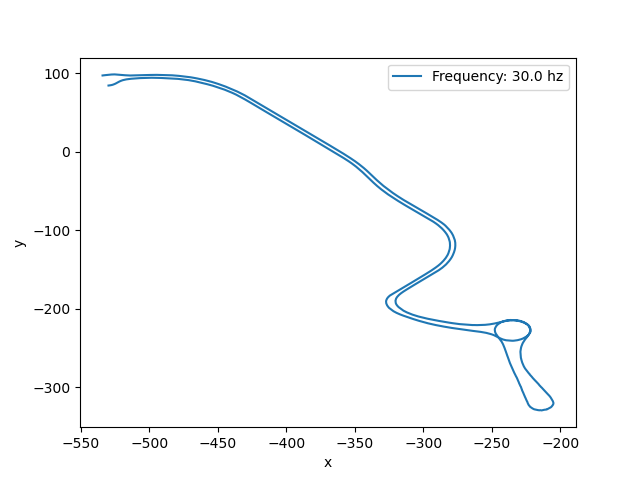
\includegraphics[scale = 0.7]{fig/gt.png}
    \end{center}
    \item Interpolation
    For computing the interpolation, we assume that the downsampled data $\{x,y\} = f(t)$, i.e., the points are equally spaced in time.
    The formulae and methods are taken from the lecture notes. Python implementation is attached as $\tt{main.py}$ file.
    \begin{enumerate}[itemsep=5ex]
      \item Linear Interpolation:
      \begin{center}
        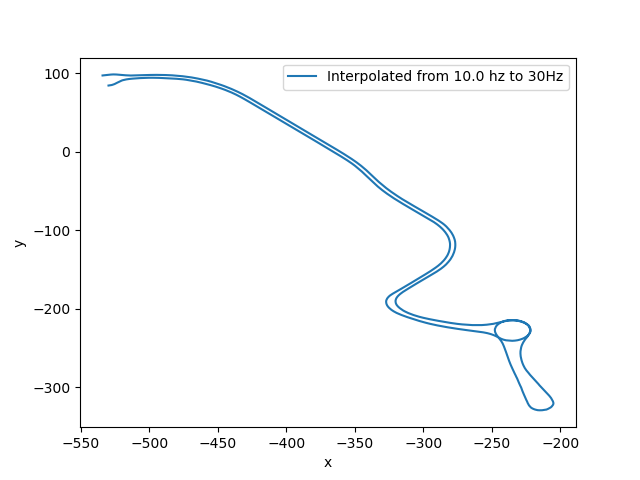
\includegraphics[width=0.32\linewidth]{fig/lin_10.png}
        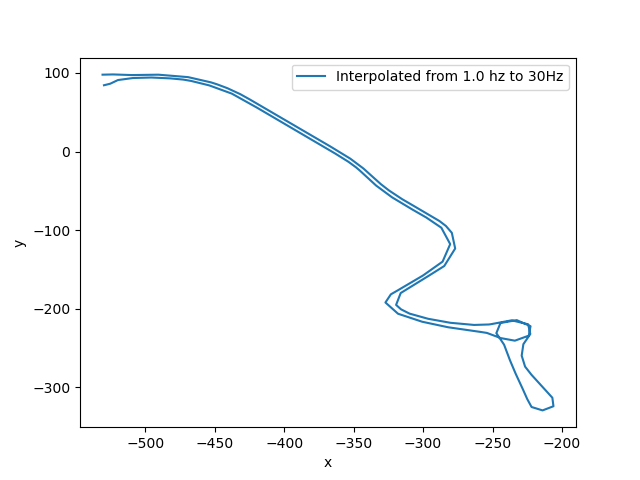
\includegraphics[width=0.32\linewidth]{fig/lin_01.png}
        \includegraphics[width=0.32\linewidth]{fig/lin_P2.png}
      \end{center}
      Linear Interpolation Error:
      \begin{center}
        \begin{tabular}{ |c|c|c|c| } 
        \hline
        \bf{Downsample freq.} & \bf{Euclidean norm error} \\
        \hline
        10Hz & 45.77 \\ 
        01Hz & 1486.57\\ 
        0.2Hz& 23702.15\\ 
        \hline
        \end{tabular}
      \end{center}
      
      \item Quadratic Interpolation:
      \begin{center}
        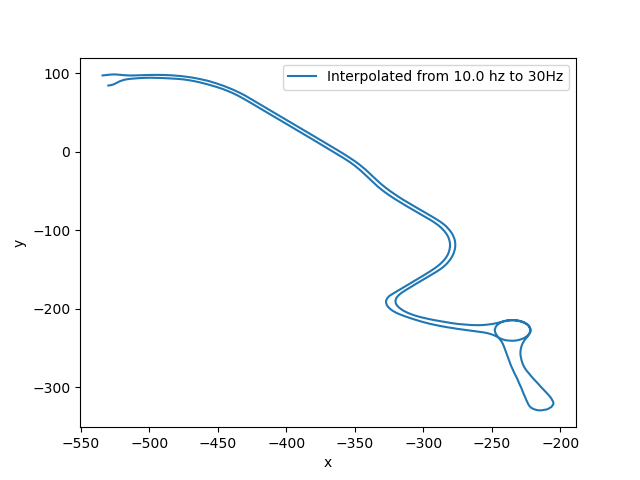
\includegraphics[width=0.32\linewidth]{fig/quad_10.png}
        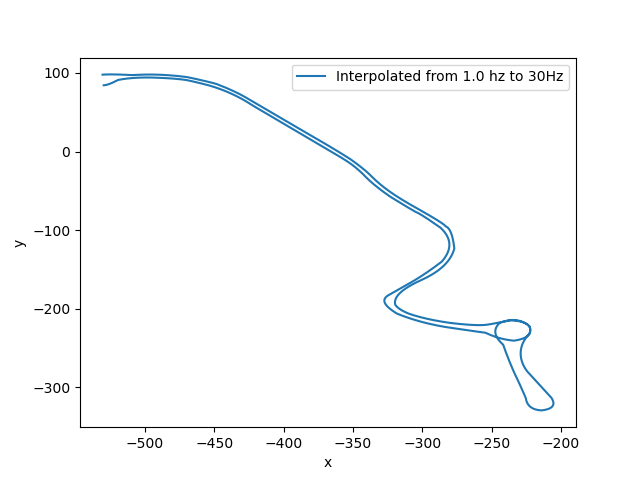
\includegraphics[width=0.32\linewidth]{fig/quad_01.png}
        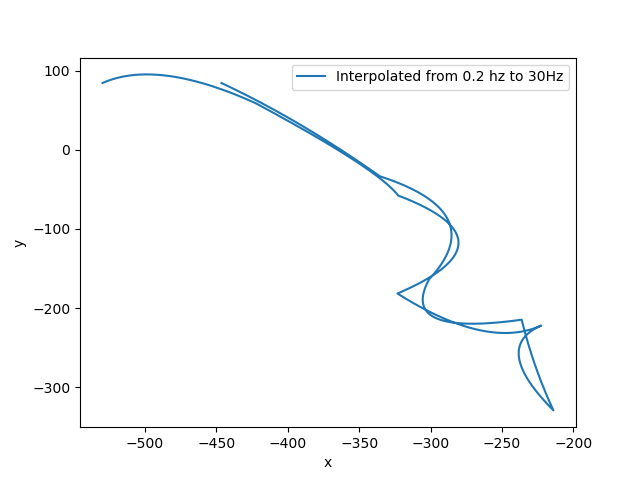
\includegraphics[width=0.32\linewidth]{fig/quad_p2.png}
      \end{center}
      Quadratic Interpolation Error:
      \begin{center}
        \begin{tabular}{ |c|c|c|c| } 
        \hline
        \bf{Downsample freq.} & \bf{Euclidean norm error} \\
        \hline
        10Hz & 46.42 \\ 
        01Hz & 876.68\\ 
        0.2Hz& 21672.22\\ 
        \hline
        \end{tabular}
      \end{center}
      \item Cubic Spline Interpolation:
      \begin{center}
        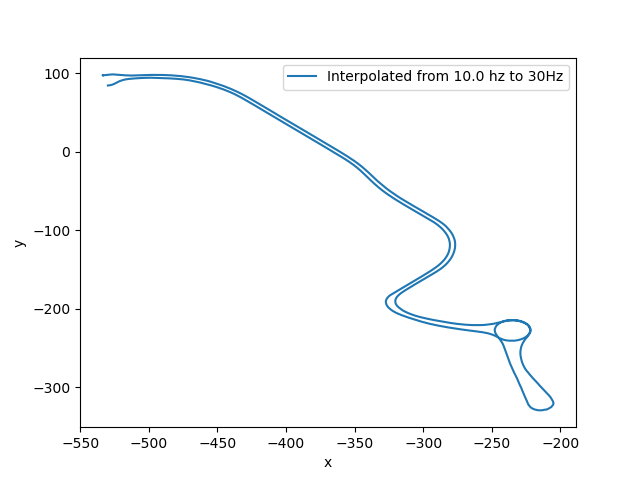
\includegraphics[width=0.32\linewidth]{fig/cub_10.png}
        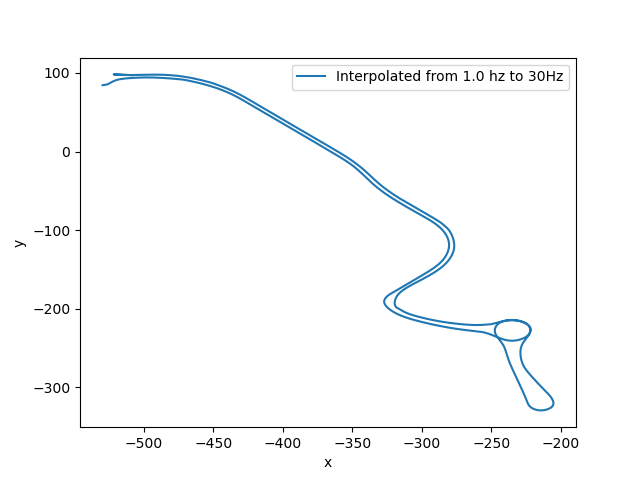
\includegraphics[width=0.32\linewidth]{fig/cub_01.png}
        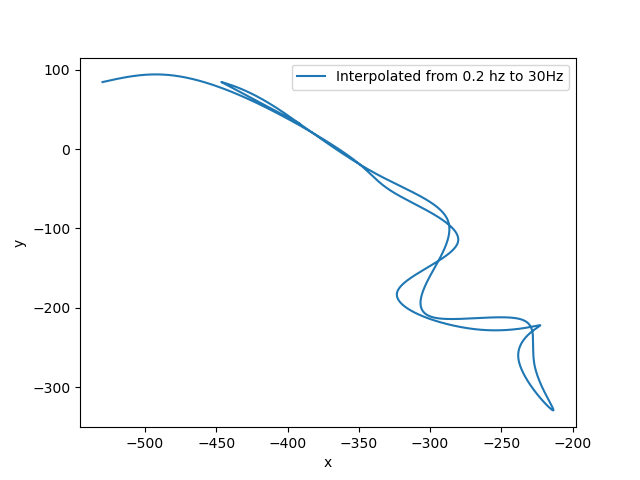
\includegraphics[width=0.32\linewidth]{fig/cub_p2.png}
      \end{center}
      Cubic Spline Interpolation Error:
      \begin{center}
        \begin{tabular}{ |c|c|c|c| } 
        \hline
        \bf{Downsample freq.} & \bf{Euclidean norm error} \\
        \hline
        10Hz & 46.27 \\ 
        01Hz & 463.28\\ 
        0.2Hz& 17534.76\\ 
        \hline
        \end{tabular}
      \end{center}
    \end{enumerate}
    \item For the 10Hz downsampling rate, there is very minute difference between the three types of interpolations (linear, quadratic and cubic spline). All look
          similar to the ground truth trajectory.
          
          As we further downsample our data, we observe that cubic spline interpolation is the most reliable with the least error, unlike linear interpolation.
          
          As the above trend continues, the difference between quadratic and cubic spline interpolation is noticeable.
          
          The low sample rate of 0.2Hz is most detrimental in case of curvatures where we are not able to capture the continuity of the trajectory. The condition aggravates
          for linear interpolation.

    \item
    In linear interpolation, we approximate a function with a straigh line and it performs better if the function has traits, which are linear.
    
    In quadratic interpolation, we approximate a function with a quadratic curve and it performs better with functions which have a curvature similar
    to a 2-degree polynomial; however, there are certain edge cases within the curve, where the function is not differetiable. It makes the changes in
    the curve abrupt, which should not be the case.
    
    Finally, we implement cubic spline interpolation, which allows us to make the curve differentiable and the edge cases are less abrupt.
    
    Hence, each interpolation would work better with functions which display similar traits for the given domain and range.

    They differ dramatically in cases of lower sampling rates, as each method interpretes the huge amount of lost information in a different way. With higher
    sampling rates, we do not see much difference.
    
  \end{enumerate}
  \item Problem 2:\\
  Since, we want 6 digit accuracy for the $cos(x)$ function, we say that our maximum error should be $10^{-6}$.\\
  The error is expressed by the following formula:
  \begin{equation}
    \mathbb{E} \leq \frac{1}{(n+1)!} \max_x{f^{n+1}(x)\prod_{i=0}^{n} (x - x_i)}, for\ x \in [0, \pi]
  \end{equation}
  where $n$ is the degree of polynomial used to interpolate the given function.

  \begin{enumerate}
    \item Linear Interpolation:
    For linear interpolation, $n=1$. Hence, using (1):
    \begin{equation}
      10^{-6} \leq \frac{1}{2!}\max_x{|\frac{d^3cos(x)}{dx^3}|}\max_x|\prod_{i=0}^{1} (x - x_i)|
    \end{equation}
    \[
      \max_x{|\frac{d^3cos(x)}{dx^3}|} = \max_x{|sin(x)|} = 1, for \ x \in [0, \pi]
    \]
    \\
    To get the max of product, we differentiate it with respect to $x$ as follows:
    \[
      \frac{d}{dx}(\prod_{i=0}^{1} (x - x_i)) = 0,
    \]
    \[
      \implies 2x - (x_0 + x_1) = 0
    \]
    \[
      \implies x = \frac{(x_0 + x_1)}{2}
    \]
    Substituting $x$ in (2):
    \[
      10^{-6} \leq \frac{1}{2!}\max|\frac{x_0 - x_1}{2}\frac{x_1 - x_0}{2}|
    \]
    Let $h = x_1 - x_0$ be the table spacing,
    \[
      10^{-6} \leq \frac{1}{2!}|\frac{-h^2}{4}|
    \]
    \[
      \implies h \geq \sqrt{8\times10^{-6}} = 0.0028
    \]
    Hence, the required table spacing is $h = 0.0028$.
    \\
    \item Quadratic Interpolation:
    For quadratic interpolation, $n=2$. Hence, using (1):
    \begin{equation}
      10^{-6} \leq \frac{1}{3!}\max_x{|\frac{d^4cos(x)}{dx^4}|}\max|\prod_{i=0}^{2} (x - x_i)|
    \end{equation}
    \[
      \max_x{|\frac{d^4cos(x)}{dx^4}|} = \max_x{|cos(x)|} = 1, for \ x \in [0, \pi]
    \]
    \\    
    To get the max of product, we differentiate it with respect to $x$ as follows:
    \[
      \frac{d}{dx}(\prod_{i=0}^{2} (x - x_i)) = 0,
    \]
    \[
      \implies x = \frac{(x_0 + x_1 + x_2)}{3}
    \]
    Substituting $x$ in (2):
    \[
      10^{-6} \leq \frac{1}{3!}\max|\frac{(x_1 - x_0) + (x_2 - x_0)}{3}\frac{(x_0 - x_1) + (x_2 - x_1)}{3}\frac{(x_0 - x_2) + (x_1 - x_2)}{3}|
    \]
    Let $h = x_1 - x_0 = x_2 - x_1$ be the table spacing,
    \[
      10^{-6} \leq \frac{1}{3!}|\frac{2h^3}{3}|
    \]
    \[
      \implies h \geq \sqrt[3]{9\times10^{-6}} = 0.0208
    \]
    Hence, the required table spacing is $h = 0.0208$.
    
    \item To get the number of entries:
    \begin{enumerate}
      \item For Linear Interpolation:
      \[
        N = \frac{\pi - 0}{h} = \frac{\pi}{0.0028} \approx 1111
      \]
      \item For Quadratic Interpolation:
      \[
        N = \frac{\pi - 0}{h} = \frac{\pi}{0.0208} \approx 152
      \]      
    \end{enumerate}
  \end{enumerate}
\end{enumerate}
\end{document}















